\eandmchapter{Roles of Engineering and Metaphysics}{The Independence and Proper Roles of Engineering and Metaphysics in Support of an Integrated Understanding of God's Creation}{Alexander R. Sich}{Franciscan University of Steubenville}

\begin{abstract}

\index{science!theoretical}
\index{science!speculative|see{science, theoretical}}
\index{science!productive}
\index{speculative science|see{science, theoretical}}
\index{productive science|see{science, productive}}
In the \textit{speculative} (or ``theoretical'') sciences---including mathematics, natural sciences, and metaphysics---the world is studied independent of human volition, calling people to recognize the truths obtained about the world as valuable in their own right. Indeed, these disciplines are ordered to ``understanding-thinking'' as an end in itself. The engineering disciplines, in contrast, are \textit{productive} sciences ordered to ``understanding-making''---not as ends in themselves but to achieve practical ends \semph{per our wills}.

\index{physics}
\index{artifact}
\index{biology}
\index{nature}
\index{natural thing|see{nature}}
Natural science and engineering focus on different subject areas. In physics all forms of natural \semph{non-living} matter in physical motion are studied by modeling ``objects'' according to mathematical formalisms while employing \semph{univocal} terms such as force, energy, mass, charge, etc. In biology all natural \semph{living things} are studied. In engineering disciplines knowledge gained from the natural sciences is applied to achieve practical ends---to the \semph{making} of artificial \semph{things} (artifacts). (Principles of motion of natural things are \semph{immanent to them}, whereas artifacts' principles of motion are imposed \semph{externally}.)

\index{science}
\index{scientism}
The knowledge obtained by the particular (or individual) natural sciences and engineering disciplines is limited because they \semph{all} presuppose certain extra-scientific concepts and principles. These concepts and principles cannot be derived from any of the natural sciences themselves, for that would be circular. Moreover, the scientific method cannot validate its own ability to guide scientists to truths about creation: it cannot be the epistemic arbiter of all knowledge---otherwise known as the non-scientific pseudo-philosophy of scientism.

\index{metaphysics}
\index{being}
\index{contingency}
\index{change}
\index{ontology}
\index{worldview}
\index{contingent being}
\index{change}
\index{philosophy of nature}
It falls to metaphysics to include the study of the most general principles common to all contingent beings---whether natures or artifacts. For example, it is not the reduced understanding of motion studied in physics through physical efficient causality that is studied within metaphysics, but all manifestations of change \semph{qua} change. Metaphysics does not ask, ``\semph{how} do objects change?'' but ``\semph{what} is change?'' In metaphysics, reality is studied in ontological terms (hence, also employing \semph{analogous} terms), for it must understand what being, change, substance, accident, cause, potency, act, essence, etc. are in their widest throw. Moreover, metaphysics cannot be reduced to a crude synonym for ``worldview'': it is a rigorous speculative science that \semph{inter alia} animates the coordinating role a realist philosophy of nature plays for the particular natural sciences and engineering.

\index{realism}
\index{philosophy of nature!realism}
\index{change}
\index{nature}
\index{methodological naturalism|see{naturalism, methodological}}
\index{naturalism!methodological}
It falls within a realist philosophy of nature to study the most common principles of the natural sciences. To provide the foundational principles which all particular sciences and engineering disciplines presuppose, there must be a way of knowing nature whose subject matter concerns the principles and causes of natural things insofar as they are natural---that is, subject to change per principles immanent to themselves. A realist philosophy of nature therefore has the same general subject matter as the natural sciences, but it applies general philosophical (rather than specific scientific) methods to study nature, and it does not suffer the operational restrictions of methodological naturalism.

\index{philosophy of science}
\index{naturalism!philosophical}
\index{philosophical naturalism|see{naturalism, philosophical}}
\index{materialism}
\index{natural philosophy}
Philosophy of nature must be distinguished from philosophy of science---the latter of which includes the study of \semph{systems of reasoning about natural things}. It must not be confused with \semph{philosophical naturalism}, nor should it be conflated with the term ``natural philosophy'' as used during the Enlightenment, whose antecedents reflect a slow, incremental drift from a unified understanding of nature into the fragmentary and highly-specified particular sciences observed today.

\end{abstract}

\section{Introduction}

\introquote{\textit{You arranged all things in measure and number and weight.}} 

\introquoteref{Wisdom of Solomon 11:20}

Metaphysics and engineering must be carefully distinguished to understand their subject matters and proper roles in support of an integrated understanding of God's Creation, and to avoid confusion that stifles such understanding, which in turn leads to an erroneous view of reality.

\index{metaphysics}
\index{cognition!metaphysics}
\index{free will}
\index{causality}
\index{phenomenology}
Today, predominate schools of philosophy are, at best, indifferent to, but more likely positively skeptical---if not openly hostile to---metaphysical thought. Metaphysics is unfortunately not understood as the classical systematic study of being as being and the properties that apply to all beings, but a grab-bag of diverse problems (e.g., free will, the existence of God, mind-body, ``eviscerated'' causality, etc.), whose only common bond is that they cannot be solved by the natural sciences, phenomenology, or other hyper-specialized disciplines.

\index{worldview}
\index{philosophy}
Perhaps more unfortunately, metaphysics is often reduced to a crude synonym for ``worldview'' or ``philosophy''---a cheap, pseudo-mystical account relegated to dime-bookstores. An examination of the conference itself will provide a backdrop for this study.  On the conference website metaphysics is described thus:

\begin{quoting}
In short, metaphysics \semph{is} about the ultimate nature of reality. It includes many aspects of reality that are generally skipped over in standard physics, such as choice, creativity, morality, aesthetics, etc. While many engineers implicitly use their understanding of metaphysics when developing solutions, our goal is to move that thinking into explicit terms, so that those parts of our understanding can be better explored and systematized. Science is often bound by a methodological disregard for anything other than efficient causes. However, as engineers, our job is to include the whole of reality, and provide solutions that incorporate our entire knowledge of reality. Therefore, this conference aims at starting the discussion of how the fields of metaphysics and engineering influence each other \citep{aboutconference}.
\end{quoting}

%Fear of oversimplification notwithstanding, I will briefly ``unpack'' this description, but later in the paper expand upon some of the particular points.
The following comments will set the stage for the discussion that follows.

\index{scientism}
\index{causation!efficient causation}
\index{causation!material causation}
\index{causation!formal causation}
\index{efficient causation|see{causation, efficient causation}}
\index{material causation|see{causation, material causation}}
\index{formal causation|see{causation, formal causation}}
\index{engineerism}
\index{artifacts}
\begin{enumerate}
\item Indeed, metaphysics is ``about'' the ultimate nature of reality, but in a qualified sense. Practitioners study the principles of all contingent existents (beings) and, hence, can support reflection upon ``choice, creativity, morality, aesthetics''{\jdots}and revealed knowledge. For example, in biology extra-mental objects known as \textit{living things} are studied; within the philosophy of nature this biological knowledge of living things is reflected on to understand what \textit{life} is; in metaphysics what \textit{beingness} is---what it means for a thing to exist---is studied, irrespective of whether the object considered is living or not, or whether the object is an extra-mental existent or a being of reason, etc.
\item This means there is no place for the study of choice (free will) in physics because physics has an altogether different subject matter: extra-mental material objects undergoing physical changes. Free will is not an object of study in the same sense that a neutrino is. If a physicist were to suggest the only types of existents are material objects and physical phenomena, or if he were to suggest free will can be ``located'' behind quantum indeterminacy, or if he were to \mbox{argue} that something can indeed come from nothing, that physicist would not be ``doing'' physics but philosophy, and bad philosophy at that.\footnote{Examples 
of scientists who stray outside their fields of competence to engage in poor philosophizing on the concept of “nothing” are Stephen Hawking \citeyearpar{hawking2012} and Lawrence M. Krauss \citeyearpar{krauss2013}. 
See also Duke University philosopher Alex Rosenberg \citeyearpar{rosenberg2013} who denies free will, denies purpose, denies human thought is “about” anything, and unabashedly promotes scientism, physicalism, and nihilism.}
\item Moreover, metaphysical categories and ``thinking'' cannot be ``move[d]{\jdots}into explicit terms, so that those parts of our understanding can be better explored and systematized.'' The methodologies and language employed by metaphysics are not those of engineering. The latter operates almost exclusively in univocal terms; the former also employs analogous terms, primarily because ``being'' is itself an analogous notion. The demand that metaphysics be reduced to ``explicit terms'' is a surreptitious reduction of the kinds of beings studied in metaphysics down to the ontological level of those beings studied by engineering.
\item The natural sciences are \textit{not} ``often bound by a methodological disregard for all but efficient causes''; they also incorporate physically-based material causes and a ``rarified'' version of the formal cause as manifested through mathematics. Moreover, the natural sciences are not constricted by a non-realist or instrumentalist interpretation of their efficacy: the natural sciences can and do provide insights into the natures of the objects being studied \textit{as actually existing}.
\item It is most manifestly not the objective or responsibility of engineering to include the whole of reality. Engineers \textit{make artifacts} based upon the application of highly focused natural scientific knowledge through refined \textit{techniques} upon existing matter. Engineering cannot be looked upon to distinguish between \textit{artifacts} and \textit{natures}, for the objects of which it is productive can \textit{only} be artifacts: engineering presupposes---even if inchoately expressed---that \textit{artifacts imitate natures}, and not the other way around. \textit{Scientism} is the pseudo-philosophical notion that the modern empirical sciences (MESs) are the epistemic arbiters of all knowledge. Imputing a similar role to engineering would result in \textit{engineergism}, which should also be avoided.
\end{enumerate}

\section[Definitions and Differences of Sciences]{Definitions and Differences of Sciences\footnote{This section summarizes salient principles presented in sections II-IV of \citet[][pp.~23--167]{adler1978}.}}

Some basic foundational questions will contribute to the manner in which knowledge is obtained in that discipline:

\begin{itemize}
\item What is ``science?''
\item What is ``engineering?''
\item What is ``metaphysics?''
\end{itemize}

A correct response to these questions---which, at the end of the day, should provide clear definitions---is part of the broader question that serves to demarcate the bounds of these disciplines responding to its own question: To what extent do each of these disciplines span the realm of human knowledge?

\index{telos}
Man is a \textit{reasoning being} as reflected in the definition (i.e., the logical genus and specific difference) which properly captures the essential aspect of what it means to be a \textit{human being}, i.e., a \textit{rational animal}---\textit{rational} because we are ``little'' \textit{logoi} created in the Image of The \textit{Logos}.
The very first sentence of Aristotle's \btitle{Metaphysics} echoes what man is by his very nature: ``All men by nature desire to know'' (Aristotle, \textit{Metaphysics}, I.980a21)\footnote{``\emph{All men by nature desire to know}. An indication of this is the delight we take in our senses; for even apart from their usefulness they are loved for themselves; and above all others the sense of sight. For not only with a view to action, but even when we are not going to do anything, we prefer sight to almost everything else. The reason is that this, most of all the senses, makes us know and brings to light many differences between things.'' (Aristotle, \textit{Metaphysics}, I.980a21)} Moreover, we as humans are commanded by Christ not to leave our brains at the door of knowing and loving God: ``And thou shalt love the Lord thy God with all thy heart, and with all thy soul, and with all thy \semph{mind}, and with all thy strength: this \semph{is} the first commandment'' (Mark 12:30 KJV also echoed in Luke 10:27). However, the \semph{kind} of thinking man undertakes differs importantly depending on the \fword{telos}---the end sought. As such, there is a crucial logical distinction based on the role of truth in all human activities, i.e., the distinction of seeing man as a knower for the sake of knowing, as a doer or ``acting individual,'' and as a maker or ``builder.''

Stated another way, the \semph{kind} of thinking man does (1) as a knower for the sake of knowing (i.e., productive of knowledge) differs from (2) the thinking done to act morally, socially, or politically (i.e., productive of actions), which differs from (3) the thinking done to make things (i.e., productive of artifacts). In the sphere of \semph{knowing}, humans are concerned with \semph{truth as truth}; in the sphere of \semph{doing} with \semph{truth as action} (characterized as good and evil, right and wrong, etc.); in the sphere of \semph{making}, with \semph{truth as beauty} (producing things that are ``well-made'').

\index{transcendentals}
\index{true|see{truth}}
\index{truth}
\index{good}
\index{goodness|see{good}}
\index{beauty}
\index{beautiful|see{beauty}}
Indeed, the \semph{true}, the \semph{good}, and the \semph{beautiful} are among those few but extremely important metaphysical terms called ``transcendentals''---terms which apply to all contingent beings to the extent they exist, and as such are not \semph{valuative} but ontological.\footnote{The transcendental terms express transcendental modes of being which, according to Fr. William Wallace, are ``coextensive with being; in them being manifests itself and reveals what it actually is. Just as being is never found without such properties, so these are inseparably bound up with one another in the sense that they include and interpenetrate each other. Consequently, according to the measure and manner in which a thing possesses being, it partakes of unity, truth, goodness; and conversely, according to the measure and manner in which a thing shares in these properties, it possesses being. This ultimately implies that subsistent being is also subsistent unity, truth, and goodness'' \citep[][p. 85]{ephil}.  In typical accounts there is the existent (\textit{ens}) itself and its essence (\textit{essentia}), then being is said to be one, good, true (\textit{unum}, \textit{bonum}, \textit{verum}) and beautiful (\textit{pulchrum}), although St. Thomas Aquinas includes two more: thing and something (\textit{res}, \textit{aliquid}) in \textit{Disputed Questions on Truth} (q.1 a 1). The transcendentals are ontologically one; thus, they are convertible: where there is truth, there is also beauty and goodness. The important point above and beyond the notion that the transcendentals are convertible and coextensive is that they are free from the limitations of particular \textit{kinds} of \textit{being}: \textit{all} contingent beings are true, good, beautiful, etc. \textit{to the extent they exist}. These terms ``transcend'' not in a ``vertical'' sense but in the ``horizontal'' sense that they apply to \textit{all} contingent beings.} 
A fly is ``beautiful,'' but not beautiful in the way people normally characterize, say, humans or roses or paintings---not in an emotional, aesthetic, quantitative, or ``valuative'' sense, but in the sense of an ontological hierarchy: a human exists ``more''---has a greater ``claim'' to existence---than a fly. It is ``better'' to exist than to not exist at all, and it is ``better'' to exist at a higher ontological level than at a lower level.\footnote{This understanding also stems from a correct rejection of the gross metaphysical error known as the \textit{univocity of being}, which holds that everything that exists ``possesses'' the same ``level'' or ``claim'' to (or mode of) existence, e.g., that the number 2 ``exists'' in the same way a carbon atom exists. Clearly, the accident of quality (e.g., ``red'') cannot exist without the more fundamental existence of the primary substance (e.g., this particular ball) in which it inheres. Perhaps more importantly, an electron does not ``enjoy'' the same level of existence as the chair under whose beingness it is subsumed, and ``design'' does not exist in the same way bacterial flagella exist.} 

A rock, in turn and in this sense, is ``less'' beautiful than a fly, but again not an emotional, aesthetic, or ``valuative'' sense. God does not ``exist''---He IS Existence Itself, without a hint of potency (hence, unchanging), utterly simple, and in that sense He is Beauty Itself.\footnote{The ultimate aim of metaphysics is knowledge of God as the human mind can acquire. Aquinas uses analogous names to give an account of the divine attributes such as wisdom, justice, mercy, being, one, true, good, etc. See \textit{Summa Theologiae} I.13.}

\index{subject matter}
\index{kind (ontological)}
\index{demarcation}
So how are the relevant portions of reality demarcated for study among the various scientific disciplines? What should distinguish the particular sciences is---employing logical terms of art---the \semph{subject matter} (sometimes called ``proper object'') studied within each (St. Thomas Aquinas, \textit{Commentary on the Posterior Analytics} [of Aristotle], Lectio 21, Caput 12, 77a36--77b15). In other words, the distinction is not principally rooted in what may be devised as an \fword{a priori} classification scheme, but in the very objects studied. The question ``what \semph{kind} of an object is that?'' should lead the distinction. For example, is a ``neutrino'' the same \semph{kind} of thing as a ``frog,'' or a ``Venus flytrap'' the same \semph{kind} of thing as a ``triangle,'' or is DNA the same \semph{kind} of thing as ``design''? What this implies, of course, is that the particular sciences by themselves cannot form a basis for those distinctions, for that would be circular reasoning.

(Brief digression: at this point the reader should sense just how different the particular sciences and metaphysics are from engineering. To repeat, the former seek knowing for its own sake; the latter seeks knowing in order to make.)

\index{science}
To help bring out the important distinctions (and hence provide a basis for classification), the sciences will be differentiated based on the subject matter and on the outcome or result. The first question must be, ``what is science?'' Classically and in its widest throw, science is `certain knowledge through causes' or `mediate intellectual knowledge obtained through demonstration.'\footnote{%
Science (Greek \textit{epistêmê}, Latin \textit{scientia}) as understood by Aristotle: \textit{in actu: Posterior Analytics}, I:2 and II:19; \textit{in actu exercito: Physics} I:1; see also Fr. William A. Wallace, \textit{The Modeling of Nature: Philosophy of Science and Philosophy of Nature in Synthesis} \citep[][p.~231]{wallace1997}; Thomas Aquinas, \textit{Commentary on the Posterior Analytics of Aristotle}, I.2.1. For Aristotle, in contrast to the modern empirical sciences, scientific knowledge is approached from the general knowledge of proximate and unreductive “wholes” from which one works toward knowledge of “parts” more “remote” to the senses. For example, we know a horse as a primary substance before we know the atoms from which the horse is constituted: there is no necessary “roadmap” that takes one from atoms “up to” the unreductive whole known as a horse, which means a horse cannot be reduced to its parts. For Aristotle, therefore, science is certain knowledge through causes and effected by demonstration. The character of \textit{certitude} flows from the use of \textit{proper} causes (neither remote effects nor causes) in an argument which supports such knowledge. Moreover, it \textit{demonstrates} (in the logical sense a \textit{sound} argument, i.e., stronger than a \textit{valid} argument which is merely a proof) \textit{through causes} (i.e., not incidental principles or elements) as middle terms of a demonstrative syllogism. In other words, the middle terms in such syllogisms “cause” new knowledge. So, “mediate intellectual knowledge obtained through demonstration” is an expanded form of the definition of science as “certain [demonstrated] knowledge through causes.”
} What this means is that theology and philosophy are also sciences, although they employ different methodologies, instrumentation, and means by which to achieve their end---truth about the real world. Just as one does not employ a telescope to study bacteria, one does not employ physics to study free will or the Transfiguration.

\index{science!theoretical}
\index{science!applied}
\index{science!methodological}
\index{science!ethics}
\index{arts}
Now that the answer to ``what does science do?'' has been introduced, names can be attached to the ``doing'': (1) the ``theoretical'' or ``speculative'' sciences are those in which truth as truth is studied; (2) in the ``applied'' sciences truth in doing/action and truth in making/beauty are studied; and (3) in the methodological sciences how human reasoning leads to truth are studied.

\index{science}
\index{abstraction level}
What exactly is studied within the particular sciences is perhaps best depicted in the diagram below which relates the two major distinctions noted above. In addition, the diagram will help distinguish the speculative (theoretical) sciences through their subject matter by means of the level of abstraction.

\begin{center}
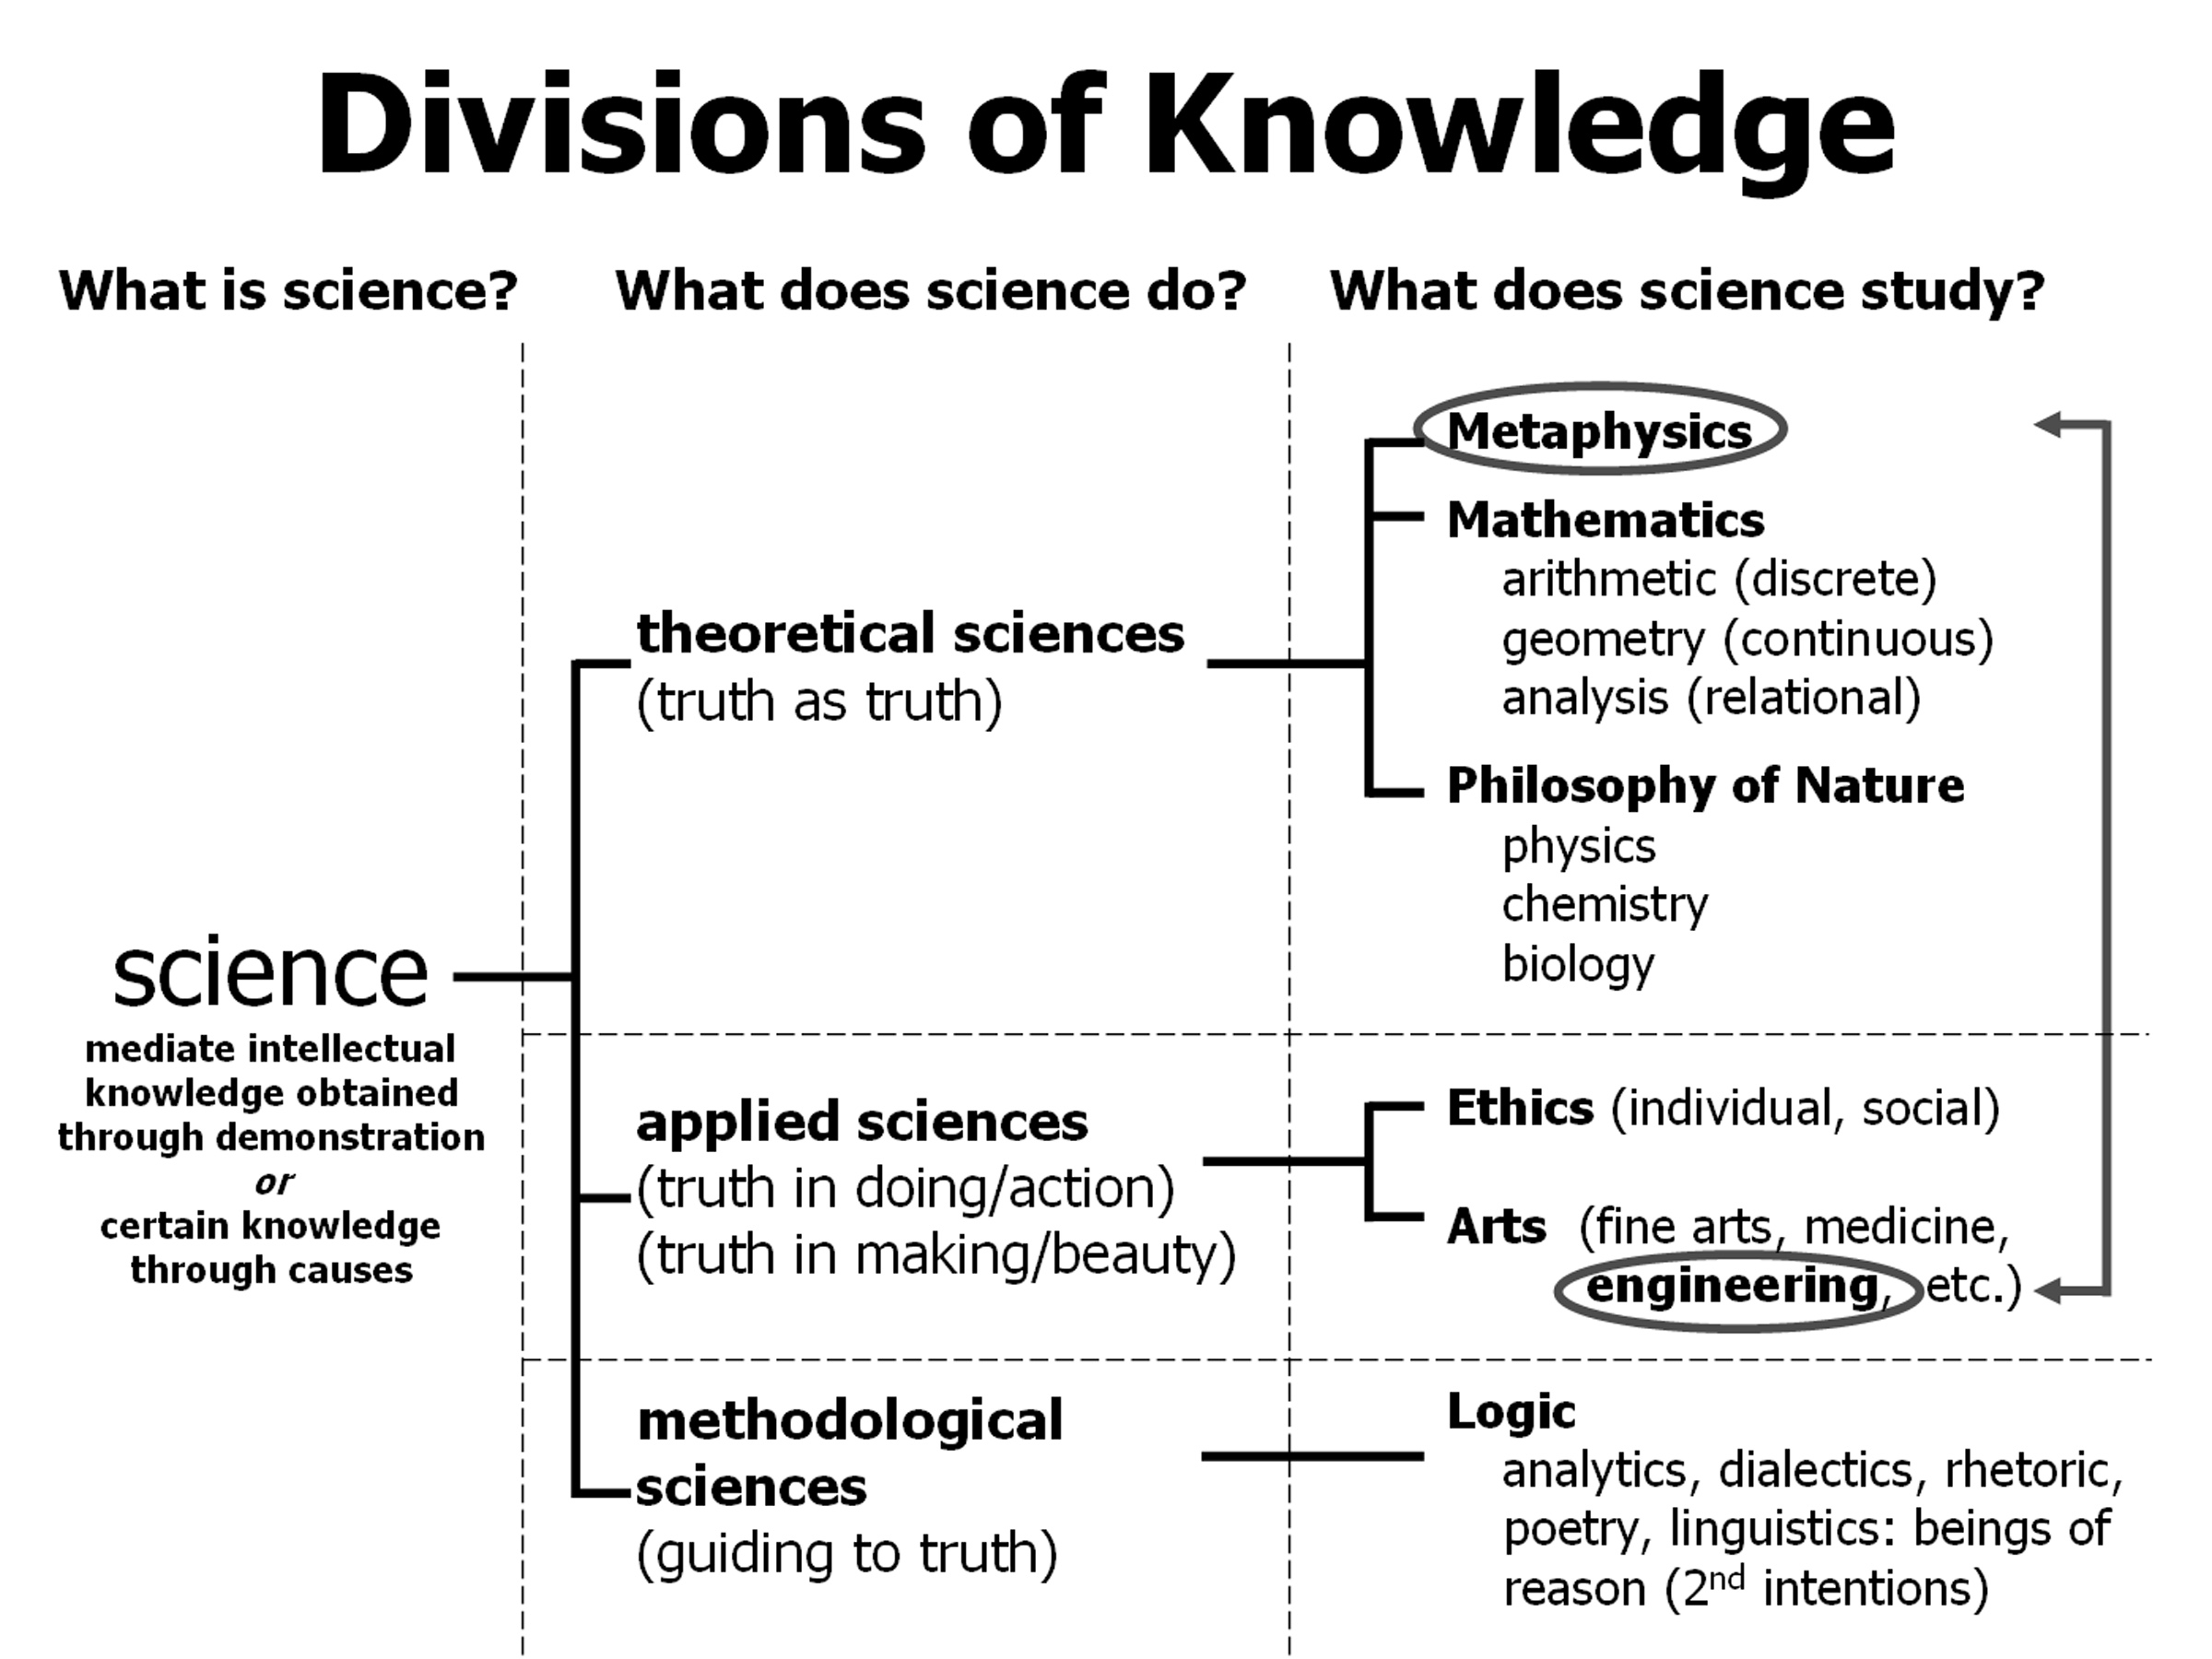
\includegraphics[scale=0.6]{sich_science_taxonomy.jpg}
\end{center}

All the particular (in the sense of ``individual'') sciences address different aspects of being. The question then becomes ``what are those \semph{fundamentally} distinguishing aspects or characteristics?''

\index{philosophy of nature}
For example, a discipline under the theoretical sciences is the \semph{philosophy of nature}, under which can in turn be distinguished each of the natural sciences:


\begin{itemize}
\item In \semph{physics} matter in physical motion is studied by modeling material ``objects'' according to mathematically-formulated deterministic mechanisms.\footnote{Note for quantum mechanics one must be careful to distinguish the mathematical formalism employed to describe the behavior of objects that are highly affected by observation (measurement) from the natures of those objects. Epistemic limitations (in measurement) currently force scientists to employ statistical mathematical formalisms to describe observed quantum phenomena, but this in no way dictates the ontological status of those phenomena. The wave equation of an electron, for example, is derived from the observation of a huge population of electrons under specific conditions, but it does not follow that an electron is---by its nature---a wave: some wave-like behavior does not imply wave-like nature. An example might clarify this: the mathematical formalism known as a normal function describing the shape of the collection of balls that have fallen through a Galton board in no way implies the balls themselves---by their nature---are ``spread out'' in space or whose motions are \semph{random} (i.e., without cause). The Copenhagen Interpretation commits a gross error in logic and scientific procedure by concluding that what cannot be measured exactly does not occur exactly: an epistemic principle was converted into an ontological principle.}
\item In \semph{chemistry} the composition, structure, and properties of matter, as well as the changes matter undergoes during chemical reactions are studied.
\item In \semph{biology} living things are studied---examining their structures, functions, growth, origin, distribution, and classification.
\end{itemize}

\index{mathematics}
\index{theology}
\index{logic}
\index{beings of reason}
\index{science!second intentions}
\semph{Mathematics}, as a science, stands apart from the natural sciences because it studies being from which all properties (philosophically: accidents) are abstracted except quantity---either discrete or continuous. In other words, mathematics studies being as quantified. \semph{Metaphysics}, a science as well, stands above all---not just abstracting but \semph{separating} everything from being except those aspects shared by \semph{all} beings. \semph{Theology} is a science: its subject matter is knowledge of God and Divine things obtained through philosophical reflection and argumentation. \semph{Logic} studies beings of reason or second intentions. It is the science that seeks knowledge for its own sake and is productive of something, for it organizes and guides reasoning to the truth. These examples aid the understanding of how levels of abstraction (from real beings to the object studied) distinguish the sciences---yielding the subject matter of each of these disciplines.


\section[The Role of Abstraction in Distinguishing the Particular Sciences]{The Role of Abstraction in Distinguishing the Particular Sciences\footnote{Many commentaries are available on the works of Aristotle and St.\ Thomas Aquinas that summarize the degrees of abstraction that distinguish the speculative sciences. See, for example, \citet[][pp.~35--36]{maritain1959} and \citet[][pp.~51--53]{velde2006}.}}
%[The Role of Abstraction]

\index{abstraction!1st level (mathematics)}
\index{category (Aristotelian)}
\index{substance!primary}
\index{substance!secondary}
\index{being!changeable (\textit{ens mobile})}
At the first level of abstraction, \semph{particular} matter is left behind to focus upon \semph{general} matter---where ``matter'' is understood in the logical sense. For example, the focus is not upon this red apple but upon the general notion of redness (physics) or the general notion of apples (biology) \semph{universally} applied to all particular objects studied. For the philosophy of nature, any particular red apple is termed a \semph{primary substance} while the universal apple is a \semph{secondary substance}; redness is an \semph{accident} (the Aristotelian category \semph{quality}) that can inhere in many different real objects. Another example is Socrates (primary substance) vs. human being (secondary substance). This first level of abstraction---generally applied to the philosophy of nature---resolves being in the sensible and the subject matter is \fword{ens mobile} (changeable being), while the individual natural sciences discriminate even further as noted below:

\begin{itemize}
\item Physics studies \semph{natural} material ``objects'' undergoing physical changes
\item Chemistry studies \semph{natural} material objects subject to electron-based interactions
\item Biology studies \semph{natural} living things
\end{itemize}

\index{artifact}
\index{nature (natural thing)}
\index{accidental unity}
``Natural''---or ``natures''---as the term is used here is not to be understood in the popular or ecological sense but as applied to those things in whom the principles for motion/change are immanent. \semph{Artifacts}, on the other hand, ultimately have their principles located externally to them. Stated philosophically, an acorn has the immanent capacity to actualize its nature into a mature oak tree.\footnote{For the distinction between natural things and artifacts: Aristotle, \btitle{Physics}, Book II, 192 b 9--18, 28. See also \citet{stump2006}.} A robot, which is technically termed an ``accidental unity,'' ultimately has its motion or change located (in the sense of \semph{explained}) as external to it: even a self-powered robot is not strictly that, for some external rational agent had to design the robot and impart upon it the ability to be self-powered.

\index{essence}
When physics studies motion,\footnote{To be quite precise, in physics one does not study motion in the same sense that in biology one does not study life. Neither motion nor life are, respectively, the objects of these sciences. In \textit{physics} one studies material \textit{things in motion}; in \textit{biology} one studies \textit{living things} (or \textit{things} that were once living). ``Things'' here are understood as real, extra-mental existents accessible to (observable by) the five external senses or the senses enhanced through instrumentation. Neither life nor motion are \textit{per se} observable by the senses: motion and life are both known to exist, but only because of reflection upon the knowledge gained through the natural sciences, and that reflection properly belongs to the philosophy of nature. See, in particular, section \ref{sec:metaphysics}, \nameref{sec:metaphysics}, page \pageref{page:motion}ff ahead.} it simplifies the things studied (termed an ``object'') in order to understand the motion, and then attempts to return to the fullness of reality by successively increasing the complexity of external influences. For example, a typical introductory freshman-level physics course may pose the following problem: an \semph{object}, for which the final position is to be determined, is hurled into the air at such-and-such a speed in such-and-such a direction. It does not matter to the study of physics whether that object is a marble, a howitzer round, or an elephant. Physics does not focus on the essence (``whatness'') or nature of the object, and it doesn't need to, nor can it. Once that basic level of motion is understood, one can then incorporate into the question other factors that will influence the motion: initial angular momentum, air resistance, expansion due to rapid heating, curvature of the earth, air currents, manufacturing flaws, etc. In fact, given time, patience, and resources, any level of precision can be attained. \semph{But}, the full ontological import and essence of the ``object'' will never be captured by physics alone---let alone by mathematics.

\index{abstraction!2nd level (mathematics)}
The second level of abstraction belongs to mathematics: all sensible aspects are left behind except the quantitative, and hence the beings studied are resolved not in the senses but in the imagination. Even highly abstract mathematical concepts (Lie groups, Fourier analysis, complex functions, etc.) must ultimately be reducible to discrete and continuous quantities abstracted from real objects. Mathematics is therefore the study of things that can be imagined and conceived without matter, not just the abstraction from the particular for the philosophy of nature and the individual natural sciences. The focus of mathematics is upon the first Aristotelian category of real being---quantity, again whether continuous (surfaces, volumes, etc.) or discrete (integers, countables, etc.) or relational (equations, inequalities, etc.).

\index{quantity!1st Aristotelian accident}
\index{being!extended in space (\textit{res extensa})}
Quantity, as the first accident of real being, is the basis for quality---the second accident of real being. For example, the average temperature of air in a room presupposes a non-point-like \fword{res extensa}---a thing spatially extended---and the ability to measure (quantify). Furthermore, quality admits of degree; quantity does not. For example, no number (quantity) of kindergarteners adds up to the intelligence (quality) of Einstein.\footnote{It also makes for good jokes among scientists, e.g., two is equal to three for large values of two.} Finally, geometry, for example, is not concerned with the question of whether a triangle (as imagined from some extra-mental object) is made of copper or of wood, but only with its absolute quantifiable nature, according to which it has three sides and three angles that add to 180 degrees in Euclidean (flat) space.

\index{abstraction!metaphysics (separation)}
\index{being!contingent}
The final level of abstraction is actually \semph{separation}: all material aspects are left behind or separated from that which can exist without matter. Angels, for example, are purely immaterial beings and as such cannot in any way be imagined, for imagination requires an image---a picture---in the mind. Metaphysical terms such as unity, substance, soul, potency, causes, etc. exist without matter as well because such concepts apply to all extra-mental existents. In metaphysics, therefore, one does not study being as changeable (philosophy of nature) or as quantifiable (mathematics) but being as being, and hence such being can only be resolved through concepts in the mind. As such, metaphysics is the study of the foundational principles of all beings---those aspects shared by \semph{all} contingent beings.

\index{ontology}
\index{metaphysics!transcendental}
In a strong sense, metaphysics is really at the heart of philosophy since it deals with the nature of reality in its widest throw. Metaphysics comprises two main areas or sub-disciplines: ontology and transcendental metaphysics. Ontology concerns itself with responding to the question ``what exists?'' while Transcendental Metaphysics concerns itself with the questions ``what is it for something to exist?,'' ``are there different modes of existence?,'' and ``if there are different modes of existence, what are the truth makers for these modes?'' 

More specifically, \semph{ontology} attempts to formulate a complete list of the fundamental categories of being, while \semph{transcendental metaphysics} concerns itself with (a) a fundamental understanding of essence, existence, nature, cause, etc., and the relationships between them, (b) the truth makers for modal claims, and (c) the transcendental attributes of being---attributes which apply to all beings simply as beings.

An example of this philosophical approach is shoes. What is common or universal to all shoes cannot be drawn or imagined. As such, there is absolutely nothing which can be sensed---and hence measured---about ``shoeness.'' When one has an idea (not image!) of what is common to all shoes, of every shape, size, color, style, etc., one has grasped \semph{conceptually} the form (formal cause---the ``whatness'')---the shoeness.

\section{Metaphysics: The Foundational Science}\label{sec:metaphysics}

\index{science!foundational (metaphysics)}
\index{science!fundamental (modern empirical)}
\index{science!particular}
So, metaphysics is the foundational philosophical discipline---quite literally \semph{the} foundational science. Whereas the modern empirical sciences (MESs) are the most fundamental form of knowledge because their objects are accessible through the senses, the MESs are neither the only form of knowledge nor the most important. All the particular (individual) sciences---including the productive sciences such as medicine and engineering and architecture---depend upon metaphysics for their ultimate presuppositions and basic principles. The particular sciences seek to understand their particular subject matters through the proximate ``ultimate'' causes within their particular domain. And, no science can prove its own proximately considered first principles. There must be one foundational science (metaphysics) which seeks to understand all reality---all contingent beings---in terms of the universal properties of being as such.

\index{change!local motion}
\index{change!most general (natures)}
For example, \semph{change}, and the species of change called ``local motion'' (translational, vibrational/oscillatory, and rotational/circular) can be illustrated through the following scenario. Suppose a group of one hundred people, chosen at random, were asked if they were seismologists that have modeled tectonic subduction zones. The expected response would be one, perhaps two. If the same group was asked if they had experienced an earthquake, the response might increase to about fifteen people. If they were asked if they know \semph{what} motion is, or at least if they had experienced it, the hands of all the people in the group would be raised. This example highlights the difference between the narrowly, yet deeply focused work of scientists, those who have had special experiences and hence knowledge, and the common knowledge shared by all individuals.

\index{change!definition}
\label{page:motion}Motion (change of position of a material object as a function of time) for a physicist is relatively easy compared to the general notion of what motion is. Physics only asks ``how do things change/move?'' whereas the philosopher must ask ``\textit{\textbf{what} is} change in its widest throw?'' Motion for the philosopher is merely a species of change, for it is not merely a metaphor to assert, ``I was \semph{moved} by the beauty of my wife.'' There was a ``before'' when I was not moved, and then there was an ``after'' when my potential to be moved was actualized into reality---the reality of actually being in love. Hence, the most general definition (i.e., not the narrow physics-based definition) of motion is ``the reduction from potency to act, insofar as the object is in potency.''\footnote{According to Aristotle, motion must be defined as ``the act [entelechy] of that which exists in potency insofar as it is such'' (\fword{actus existentis in potentia secundum quod huiusmodi}) (\btitle{Physics} 3.2, 201a27--29).} It is this general definition---based upon common experience accessible to all---that provides the foundation for physicists to do their good, mathematically described work. Change had to be understood in its widest, most general throw before physics could narrow that understanding of change to study material objects in physical motion.

So, the three speculative sciences can be defined as follows:

\begin{itemize}
\item \semph{Physics} includes the study of those things (material objects and physical phenomena) that have separate substantial (real, i.e., extra-mental) existence but are subject to change.
\item \semph{Mathematics} includes the study of those things that are free from change but which do not have separate substantial (real, i.e., extra-mental) existence: they exist only as distinguishable aspects of concrete realities, e.g., a tire's shape is a circle, the statistical distribution of students' test scores is described by a normal curve, etc.
\item \semph{Metaphysics} includes the study of those things that have separate substantial existence but are free from change---primarily the study of substances (as they are the primary mode of being); in other words, what aspects do all substances share?
\end{itemize}

\section{Quo Vadis, Engineering?}

The metaphysician asks, ``What is motion?'' The physicists asks, ``How do levers move under the influence of external forces?'' The engineer asks, ``How do I construct a structurally sound bridge that will not move (within set parameters) under the influence of external forces?'' The differences between the questions asked and hence the objects studied by these disciplines are profound.

\index{science!speculative (theoretical)}
\index{science!applied (ethics, arts)}
The goal of the speculative (theoretical or ``pure'') sciences is to conform one's mind to reality. The goal of the applied sciences is to conform one's actions to reality, and therefore by them know (a) which actions conform to reality, (b) what ought to be done, and (c) how and why one should act.

\index{philosophy!moral}
\index{engineering!productive of artifacts}
In fact, the study of the applied sciences can only be successful to the extent the pure sciences are incorporated. Ethics or moral philosophy answers the questions, ``what should humans do'' and ``why?'' The arts (including engineering as productive of ARTifacts) are subordinate to ethics. Engineers must first decide what ought to be done (which implies knowing why). Then and only then may they enter into the details of how to do it. For example, knowing how to abort a child cannot trump knowing whether or not one should do so. Through science and technology, weapons of mass destruction in Iran can be detected through remote sensing. But no natural scientific, technological, or engineering discipline can then determine what should be done about those weapons.

The applied sciences are subordinate to the speculative sciences as the speculative sciences are subordinate to the science that provides their principles---metaphysics. The knowledge obtained by the natural sciences must precede the application of the knowledge through engineering, and in that sense engineering is subordinate to the natural sciences as well.

Engineering can now be examined according to its relationship to the speculative sciences.

\begin{itemize}
\item \semph{Metaphysics} is the study of being as being.
\item \index{science!modern empirical} The \semph{modern empirical sciences} are the studies of the metrical properties (quantified observables) of changeable, material objects---objects particular to each natural science.
\item \index{philosophy of nature} The \semph{philosophy of nature} stands between these two disciplines as the study of all changeable beings---of the general properties of all real (extra-mental, substantial and accidental) existents.
\item The \semph{engineering disciplines} apply the knowledge gained from the natural sciences to achieve practical ends---to the making of artificial things (artifacts---\semph{not} natures).
\item \index{philosophy of science!methodological epistemology} The \semph{philosophy of science} is the study of systems of reasoning (methodological epistemology) of natural things.
\end{itemize}

So, metaphysics is ultimately connected to engineering because it includes the study of the first causes and principles of all beings---including those things studied by the modern empirical sciences and engineering.

However, the modern empirical sciences are ``closer'' to metaphysics because

\begin{enumerate}
\item They are speculative (theoretical) in the same way metaphysics is.
\item The modern empirical sciences provide real-world knowledge for reflection within metaphysics.
\item Metaphysics, through natural philosophy, provides the modern empirical sciences with foundational (proximate ``first'') principles.
\end{enumerate}

In contrast, engineering is ``located'' further from metaphysics because

\begin{enumerate}
\item It is applied knowledge (productive of artifacts) rather than speculative.
\item It depends upon the MESs to provide knowledge of the real world.
\item It provides metaphysics no direct substantive knowledge of the real world upon which to reflect.
\item It is subject to the constraints of the practical sciences (e.g., ethics).
\item Metaphysics, through the philosophy of nature and the modern empirical sciences, provides engineering with foundational principles.
\end{enumerate}

\index{technology!techne (artifact)}
Productive reasoning involves having what one might be tempted to call ``creative'' ideas. In fact, productive ideas are based upon some understanding of the forms that matter can take, supplemented by imaginative thinking about such details as sizes, shapes, and configurations. Scientific knowledge can indeed be applied productively: scientific knowledge, through \semph{technology}, provides the skills and power to produce things.

But the philosophical reflection that improves the common-sense grasp of the physical world provides neither the skill nor the power to produce anything. Philosophy bakes no cakes and builds no bridges. So, is it ``useless'' in the Marxist sense? No. Echoing more strongly a previous point, philosophical knowledge lays the foundations of thinking and can be ``used'' to direct lives and manage societies: philosophy animates for the sake of doing---not directly for the sake of making, which is why \semph{making} must be subordinate to \semph{doing}.

\index{artifact!art imitates nature (Aristotle)}
\index{nature!natural thing!art imitates nature (Aristotle)}
There is also an analogical connection of metaphysics to engineering insofar as metaphysicians can draw analogies from the way things are made and function to make inferences about those things that cannot change. This reflects Aristotle's crucially important principle: \semph{Art(ifact) imitates nature}, and not the other way around.

\index{telos}
\index{reasoning!productive}
\index{reasoning!speculative}
To anticipate a possible criticism: some may point to the Ancient Egyptians as an example of those who did not know physics yet built the pyramids and statues, or Ancient Romans who also did not know physics yet built roads and aqueducts, so that engineering \semph{can} precede science. This is a misunderstanding of the principle. In the order of knowing, the builder must first understand---even if inchoately---that rocks fall when released and crumble when too high an external load is imposed. Such knowledge must precede the application of that knowledge. To build something is not to do engineering, in the same sense that technology cannot be equated to science. To categorize the people of those times as scientists or engineers is actually incorrect if science and engineering are understood to be what they are to moderns, unless one does so analogously. This is not to suggest that engineering does not inform the natural sciences---it does quite significantly. However, there is \semph{no reason whatsoever} for engineering to explore physical reality other than to \semph{make} something---an artifact. If engineering's goal is simply to know, then it is no longer engineering but physics or chemistry or whatever natural science. Engineering's \fword{telos}---its end or goal---for knowing reality is to make something, not to know simply for the sake of knowing.

\section{A Case Study in the Failure to Properly Distinguish: Intelligent Design}
%[A Case Study]

\index{reductionism!mechanistic}
A mistake often made is to forget (or neglect, perhaps even intentionally) this principle, and hence to fall into one of the most common errors: the fallacy that nature imitates art(ifact)---the ``mechanistic'' reductionist error shared by Intelligent Design and DarwinISM.\footnote{%
Intelligent Design proponents have attempted to deny their project is mechanistic in its view of living organisms or their constituent systems and parts, but in doing so they appear to miss the \mbox{artifact/nature} distinction, which is not so much a characterization of living things as machines (although some do make this error) but more deeply what is meant by mechanism is a lack of immanent powers based on living things being \textit{per se} natures, and that therefore descent with modification must somehow be “guided” by an \textit{external} artificer rather than having the ability to evolve on their own. See, for example, Logan Paul Gage \citeyearpar{gage2010} and Jay W. Richards \citeyearpar{richards2010b}.
Note that these gentlemen believe (as do most Intelligent Design proponents) that “design” can be empirically detected, and hence is something directly accessible to the natural sciences. It is this notion that animates the Intelligent Design movement’s desire to inject its arguments into the biology classroom. If, on the other hand, Intelligent Design is correctly understood as a philosophical interpretation of scientific findings, the project must seek another venue other than biology classrooms.
} Consider the following claims:

\begin{enumerate}
\item \index{Behe, Michael} Intelligent Design proponent Michael Behe: ``Modern science reveals the \semph{cell is a} sophisticated, automated, nanoscale \semph{factory}'' \citep{beheinterview} [emphasis added].
\item \index{Alberts, Bruce} Darwinist Bruce Alberts: ``The entire \semph{cell can be viewed as a factory} that contains an elaborate network of interlocking assembly lines, each of which is composed of a set of large protein machines.{\jdots}Why do we call the large protein assemblies that underlie cell function protein \emph{machines}? Precisely because, like machines invented by humans to deal efficiently with the macroscopic world, these protein assemblies contain highly coordinated moving parts'' \citep[][p.~291]{balberts} [emphasis added].
\end{enumerate}

This is muddled thinking that flips reality on its head.  Behe's claim is all the worse because it is a categorical assertion, while Alberts at least qualifies his claim with ``can be viewed as.''

\index{bacterial flagellum}
\index{cell!natural thing}
\index{motor!art}
The nature or essence of a bacterial flagellum, for example, might be considered from the \semph{artificial} (note the root ``artifact'') perspective as that of a motor (a machine---an accidental unity) \semph{but only if considered in isolation from the cell}.\footnote{The point of the flagellum ``considered \semph{in isolation} from the cell'' is also important because it highlights another form of reductionism in Behe's thinking. To study most of the aspects of a bacterial flagellum (and certainly to study the components of the flagellum and their properties), the cell must be destroyed (Nature must not only be interrogated but tortured as well--harkening back to Francis Bacon's \fword{novus ordo seclorum} control over Nature), i.e., the flagellum is studied in a pathological state removed from the \semph{substance} known as the bacterial cell.} However, it is not Behe's empirical observations that indicate to him that the flagellum is a motor: he drew upon empirical observations to reason to the intelligible aspect of that thing known through the universal concept of ``motor,'' i.e., it required an immaterial nous (intelligent agent) to ``know'' the immaterial intelligible aspect of that particular biological system.

\index{per accidens@\textit{per accidens}}
\index{telos}
\index{concept!universal}
\index{functionality}
Ric Machuga pointedly explains Behe and Dembski's attempts to quantify an object's form (formal cause or specificity) and \textit{telos} (final cause or function) by providing the example of pincers. Neither mathematics nor the natural sciences can explain what the tweezers in my hand, the pliers in my tool box, the bigger pliers in my plumber's tool box, the pincers of a lobster's claw, the forceps of a surgeon, the mandibles of a bull ant, the jaw of a human being, or a fireman's ``jaws of life'' are. Yet, any intelligent agent can explain that all these examples are understood by the \semph{universal (i.e., not concrete and hence immaterial) concept} of a compound lever. There is \semph{nothing} about \semph{what} a compound lever \semph{is} that physics or mechanical engineering can tell anyone---apart from \semph{how} one works: the moment arms involved, the pressure applied at the point of contact, the position of the fulcrum, etc. Natural philosophy, on the other hand, not only permits one to ``see'' the \fword{quiddity} (``whatness'') of the object, but in the list provided it can distinguish between the three examples of \fword{per se} unities and the five examples of \fword{per accidens} unities. Machuga correctly concludes: ``The only thing all pincers have in common is an intended purpose, design, or function---in short, a form. While quantifiable shapes can be the embodiment of forms, no form can be reduced to a quantifiable shape'' \cite[p.~162]{machuga}.\footnote{Note for pedagogical reasons Machuga uses the term ``shape'' to capture all nine accidents (Aristotelian categories) of real being: {``}`Shape,' as we are using the term, refers to the totality of a thing's physically quantifiable properties, i.e., its physical shape and size, height, weight, chemical composition, etc., in its most complete description.{\jdots}It is what the sciences study'' \citep[][p.~27]{machuga}.}

\index{design}
\index{Intelligent Design}
While provocative, it is nonetheless true: Intelligent Design is neither a science nor engineering. 
Intelligent Design is a philosophical interpretation of scientific findings with theological implications,\footnote{%
See, among many examples, the subtitle of the book and the entire first chapter of William Dembski, \textit{Intelligent Design: The Bridge Between Science \& Theology} \citeyearpar[][pp.~25--48]{dembski2002}; “At the same time, contemporary ID arguments represent a return to a very traditional and biblical way of speaking” in \citet[][p.~250]{richards2010b}.
}
which the following example will help clarify.
Physicists inferred the existence of a material object---the neutrino---from physical observables, i.e., from the apparent violation of conservation of energy and angular momentum in beta decay processes. Intelligent Design theorists attempt to infer the existence of ``design'' and hence a designer. But this, of course, begs the question: Is design the same ontological kind of thing as a neutrino? No, for unless one is a materialist or other such reductionist (which is a hidden irony of Intelligent Design), design is a very different kind of thing than a neutrino.  This, in turn, then demands a very different \semph{kind of science} to study design---not a natural science, but a philosophical science.

This confusion arises precisely because Intelligent Design proponents fail to distinguish properly their subject matter, i.e., they haven't asked the question: ``Is a neutrino the same \semph{kind} of thing as `design?'{''} Since Intelligent Design proponents ontologically ``flatland'' (or ``domesticate'') design down to the level of material objects, they therefore attempt to measure and quantify formal and final causality. And, the theory also unnecessarily pits efficient causality against final causality.

The following may help shed some light on the situation:
\begin{enumerate}
\item From sensory-accessible data (effects) one can \semph{infer} (inductively reason) to the existence of an object \semph{as the cause of the effects}, whose existence can then be verified directly through the senses (or senses enhanced with instrumentation). The character of such an inference is \semph{natural scientific}, and an example of such an object is the neutrino.
\item From sensory-accessible data (effects) one can \semph{infer} (inductively reason) to the existence of an object \semph{as the cause of the effects}, whose existence can \semph{not} be verified directly through the senses, but which must be argued to through \semph{philosophical inference} (philosophically if rigorously undertaken, or at least ``recognized'' if not). Examples include ``objects'' such as design and intelligence.
\item From sensory-accessible data (effects) one can \semph{infer} (inductively reason) to the Pure Act of Existence (\semph{Ipsum esse subsistens}) or Ultimate Cause of all, but only through \semph{metaphysical inference}.
\end{enumerate}

What Intelligent Design attempts to do is bypass philosophical inference (to ``obtain'' design) and metaphysical inference (to ``obtain'' God). This is not possible: there is no way to argue \textit{directly} through the natural sciences to ``design,'' and much less so to God. The only possible means by which we can reason to the Existence of Pure Existence (God) is an argument that (a) begins with sensory-accessible effects and then argues through metaphysical reflection to higher verities (design), which culminate in the Ultimate Cause (God).

\index{abstraction}
Design is an abstraction based on sensory observations, and philosophical arguments are needed to infer to its existence, just like philosophical arguments are used to support the efficacy of scientific method. A neutrino, on the other hand, is not an abstraction; it is a real, substantive, extra-mental material object. Design is a combination of formal causality (whatness) and final causality (function or ``for what'') that partly explains the existence of artifacts---\semph{not} natural things.

\index{functionality!mathematically ambiguous}
\index{mathematics}
\textit{Functionality} or ``irreducible complexity''\footnote{Behe defines an irreducibly complex system as one “composed of several well-matched, interacting parts that contribute to the basic function, wherein the removal of any one of the parts causes the system to effectively cease functioning” \citep[][p.~39]{behe2006}.} as understood by Michael Behe is, in reality, mathematically ambiguous, and in no way can it be measured---despite protestations to the contrary. Functionality implies a \textit{telos}---a “for whatness” or final cause, which is neither a subject matter (formal object) nor material object studied by any of the modern empirical sciences.  To repeat Machuga's point above, even if one considers a pair of pliers, a nut cracker, an insect's mandibles, and a lobster claw, as having one and the same \textit{functionality} applied to different situations (to hold tight and possibly crush an object), their complexities vary widely. Which of these objects has more ``\textit{functionally} specified information''? Stephen Meyers explicitly claims that ``Dembski's theory{\jdots}applies to any system that has large amounts of such functional information'' \cite[p.~372]{sigcell}. What does  ``functional information'' mean? Are jaws-of-life more \textit{functional} than a pair of household pliers, or are they simply more \textit{complex}?  How exactly is one to measure---literally to quantify by means of a metric---the differences in function between the physical examples above? Again, one cannot mathematically distinguish functions. The function is the same for all the examples above (and many more), while their mathematically describable complexities (through the correlation of sensory-accessible properties into mathematical formalisms) vary widely.  Complexity and information are quantifiable, while functionality and essence (meaning) are not.

\index{specified complexity!mathematically ambiguous}
Similarly, what a thing is---or, to employ William Dembski's term, its ``specified complexity''\footnote{For a fair summary, including definitions, mathematical treatment, criticisms, and references, see \citet{scwp}.}---is also mathematically ambiguous, and Intelligent Design actually fails to properly distinguish ``information'' (which is measurable) from ``meaning'' (which is not measurable).  Intelligent Design appears to conflate the two. To be ``specified'' is to be a \textit{specific} thing, to be an actualized existent---a \textit{primary substance} that is \textit{understood} or intelligible or whose whatness is known. In other words, it is the formal cause of a thing Dembski is attempting---and failing---to quantify.  If the Ukrainian word \foreignlanguage{russian}{ЧЕРВОНЕ} is written with smoke in the sky in all--caps, bold--faced, with letters each 100 meters tall, and if the English word ``red'' is printed in small--case 8--point font size, these two words have (gender signification notwithstanding in Ukrainian) \semph{precisely the same meaning}.\footnote{Both words have differing and measurable ``amounts'' of information which can be understood as reflecting complexity. Yet, both words have exactly the same specification (intentionality): ``redness.'' What metric has Dembski proposed to measure and distinguish \semph{per se} specification? What exactly does it mean for something to be \semph{metrically} ``more'' or ``less'' specified? The ``meaning'' of something is expressed through a definition (genus and specific difference) which yields the \semph{essence}---\textit{what} something is, which is utterly inaccessible to being measured in any way. The form is the philosophically causal explanation of \semph{what} something is, and it \semph{informs} our knowing \semph{what} that object is. The \semph{essence} is the actual \semph{whatness} of the object expressed in a definition: it is what our minds ``become'' when we come to know the object. We know the meaning---what something is---when our immaterial minds are informed \semph{essentially} to ``become'' that object.} Yet, the information content required to represent the physical aspects of these two words in a computer's memory would be very different.  Nonetheless, Dembski claims (which the scientific community correctly rejects, even as it only partly understands why): ``If there is a way to \semph{detect} design, specified complexity is it'' \citep[][p.~19]{dembskinfl} (emphasis added).\footnote{``Intelligence'' is not an object inferred to directly \semph{through} the natural sciences but \semph{through} philosophical reflection. All people recognize intelligence immediately when they ``see'' it. Yet, that ``recognition'' is not ``seen'' optically but by the operation of the mind above and beyond the sensory-accessible import. When formalized, the ``seeing'' of ``intelligence'' is properly called ``philosophical reflection.''}

Note also the apparent conflation of the terms ``detect'' and ``infer'': if design is ``detectable,'' then direct sensory access (or senses enhanced through instrumentation) is possible; if design is ``inferred,'' then that inference must be \semph{philosophical} given the \semph{kind} of thing design is, as noted earlier. If Intelligent Design is to be considered part of the natural sciences, it must be evaluated on its scientific merits, for which the track record (so far) has not been very good. If Intelligent Design is a philosophical interpretation of scientific findings, it has no more place in the biology classroom than DarwinISM does, and it must be evaluated on its philosophical merits.

\index{nature!natural thing}
\index{artifact}
Finally, the theory of Intelligent Design presupposes that living organisms are artifacts with externally imposed functionality and form. These organisms are then implicitly viewed as passive, mechanistic receptors of an occasionalist designer's tinkering.\footnote{With the goal of reconciling Intelligent Design with Thomism, several authors have attempted to address these issues in Jay Richards, \btitle{God and Evolution} (\citeyear{richards2010}), chapters 9--13. Such attempts have not met with much success, in part because a number of questionable claims that are made. These claims merit a rigorous response which, unfortunately, is outside the immediate scope of this paper.  For extended accounts criticizing the attempted reconciliation of Intelligent Design with Thomism, see Edward Feser.  For instance, \citet[][pp.~724,~745]{feser2013} gently chastises Jay Richards for suggesting Aquinas' views are close to those of William Paley and points to why Thomists are generally strongly opposed to Intelligent Design.  In addition to his published works, Feser maintains a blog that often covers similar subjects at http://edwardfeser.blogspot.com/.} 
As such, it fails to consider the Biblical account that God does not ``make'' individual things in nature like some Cosmic Artificer. Rather, God \semph{creates and maintains in existence} individual natures---natures which actualize, through their immanent capacities or powers---to perfections (understood philosophically) like the earlier example of the acorn growing into a mature oak tree: God doesn't ``make'' oak trees (note the inherent engineering reductionism of a natural thing to an artifact), acorns ``make'' oak trees. As reflected in Genesis 1:11--24 (KJV), ``the \semph{earth} brought forth'' and ``the \semph{waters} brought forth''. Intelligent Design demotes God's timeless, existence-sustaining creative act to some ``thing'' accessible to natural scientific inquiry.

\index{God!domestication of}
\index{God!cause among causes}
\index{God!being among beings}
At the end of the day, Intelligent Design claims that “design” and “intelligence” are “empirically detectable,”\footnote{%
“This chapter argues that God’s design is also accessible to scientific inquiry. The crucial point of this chapter is that design is empirically detectable, that is, we can detect it through observation” \citep[][p.~17]{dembski2002}
} and that by strong implication the existence of God can be inferred, never quite coming clean on the precise character of the inference (explained above). This is what is meant by Intelligent Design seeking direct\footnote{%
The previous footnote provides only one example of Dembski’s claim that “God’s design” is directly empirically detectable (that is, “we can detect it through observation”) to the natural sciences, and yet in other places he denies this \citep[][pp.~107--108]{dembski2002}. See also \citet[][p.~205]{richards2010c}:
“Most ID arguments are consistent with a variety of views about how and when God acts in nature. In fact, ID arguments are not explicitly theological. One could pursue research within an ID framework without ever asking follow-up questions; nevertheless, these arguments have positive theological implications. As a result, they can be used to construct arguments for God’s existence.”
} access to God’s existence by means of natural scientific means: God is seen as an \textit{external} ``guider'' of natural selection, which reflects an occassionalist notion of the source of actions of biological organisms. In other words, God is “domesticated” down to being a cause among causes.


As St. Paul instructs, because human beings are by nature rational animals, humans are capable of knowing ``God's eternal power and divinity'' from ``the things He has made'' (Romans 1:19--20 NASB), i.e., by the light of human reason alone:

\begin{quoting}
For what can be known about God is evident to [the wicked], because God made it \semph{evident} to them. Ever since the creation of the world, His \semph{invisible} attributes of eternal power and divinity have been able to be \semph{understood and perceived} in what He has made.'' (emphasis added)
\end{quoting}

The knowledge presupposed by St. Paul in this passage cannot possibly be of beautiful galactic nebula, bacterial flagella, cosmic fine-tuning, or engineering system analysis of cell processes---there were no modern empirical sciences at that time! Rather, this knowledge must be grounded in pre-scientific common experience and philosophical reflection animated by the presuppositions and intellectual habits whose origin is in a Christian world view.

\index{design}
\index{reductionism}
\index{Intelligent Design}
One would have to be out of one's mind to deny design in the universe. But, the reductionist view of ``design'' proffered by Intelligent Design proponents and ``design'' as understood by critically thinking philosophers are two different things. 
Reason alone and independently (as well as faith alone) can lead us to knowledge of the ``existence'' of Pure Existence Itself (``I AM THAT I AM,'' Exodus 3:14, KJV), i.e., to knowledge of the ``existence'' of the Creator. But, for the former the path is \semph{through} metaphysical reflection \semph{starting from} the natural sciences (or engineering or general observations). The former establishes a ``that'' for ``existence'' (the so-called god of the philosophers), while the latter establishes the relational ``who'' and is the basis for the trust known as ``faith'' in \semph{the} God.

No amount of empirical data can defeat a metaphysical proof or principle. Clearly, empirical data, scientific theories, and engineering expertise \textit{inform} metaphysical reasoning. But such reasoning is impervious to empirical falsification—similar to a mathematical theorem not being falsifiable by any empirical data. For example, no new empirical data will ever alter the fact that in the context of Euclidean (flat) geometry, the sum of all interior angles of any triangle adds to 180 degrees. Moreover, no new empirical data will ever defeat the Principle of Non-Contradiction, poor philosophizing on the part of certain quantum physicists notwithstanding.


\index{philosophical naturalism}
\index{scientism}
\index{Intelligent Design}
No empirical data or scientific theories exist in a vacuum: there is no ``preferred'' metaphysical interpretation attached. Yet, there must be interpretations. Whether implicitly or explicitly, secularist scientists embrace the notions of ``philosophical'' naturalism and materialism as animated by scientism. To counter this, the Intelligent Design movement cannot hope to misappropriate science, or especially to find a ``new home,'' in engineering. It must adopt a realist philosophy of nature. That is where the real battle for the mind is fought---not in or through the natural sciences. What this implies, of course, is that Intelligent Design proponents must face some deep soul-searching to realize Intelligent Design does not belong in the biology classroom any more than DarwinISM does. That is the only way the Intelligent Design movement will reclaim the high ground, and only then will it be unstoppable.

\index{science!subject matter}
The failure to distinguish the proper roles and subject matters studied in the natural sciences, metaphysics, and engineering will only lead to confusion---of which Intelligent Design and DarwinISM are only two unfortunate examples.\footnote{See \citet[][p.~372]{sigcell} for an example.} However, when these disciplines are respected and their differences celebrated (a tuba would sound ugly usurping the part of a piccolo), i.e., if they are permitted to operate as a symphony productive of truth---with the particular science as the individual instruments, metaphysics as the conductor, and God as the composer---the music would, indeed, be Divinely beautiful.

\eandmbibliography{SichLibrary}
